\documentclass{exos}
\usepackage{main}

\title{Exercices : Partitions de l'univers}
\author{Première Spécialité Mathématiques}
\date{Chapitre 6 Partie 3.2}

\begin{document}
\maketitle
\begin{minipage}[t]{0.45\textwidth}
\begin{center}
\textbf{Partitions de l'univers}
\end{center}
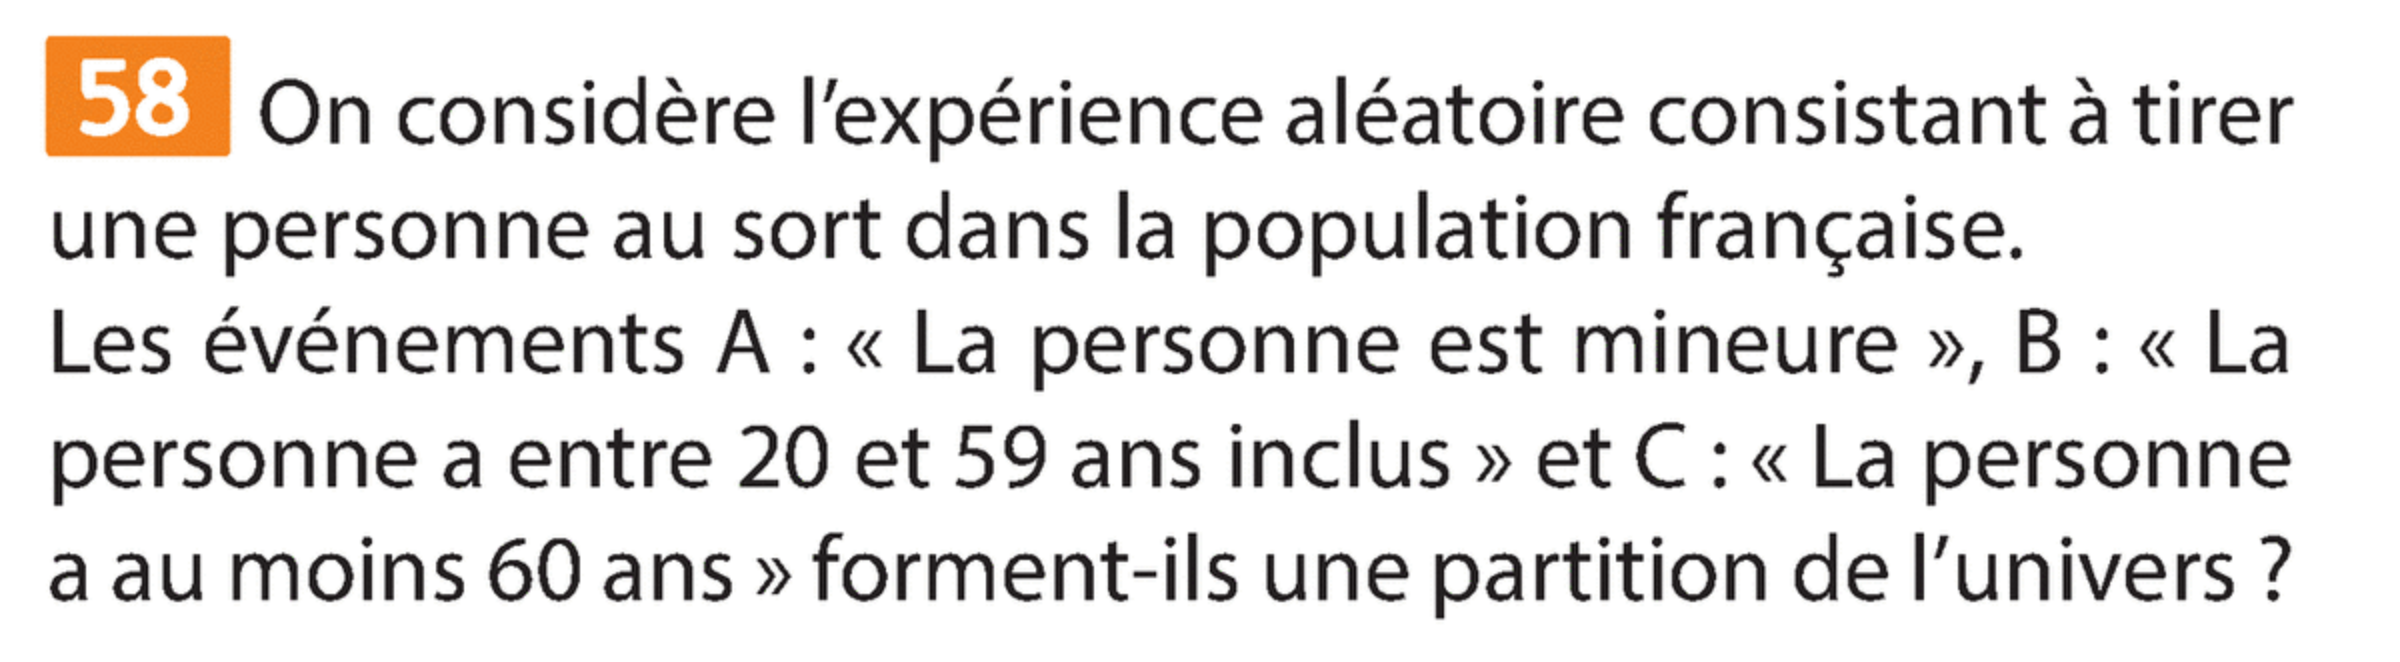
\includegraphics[width=\textwidth]{Exo_58.png}
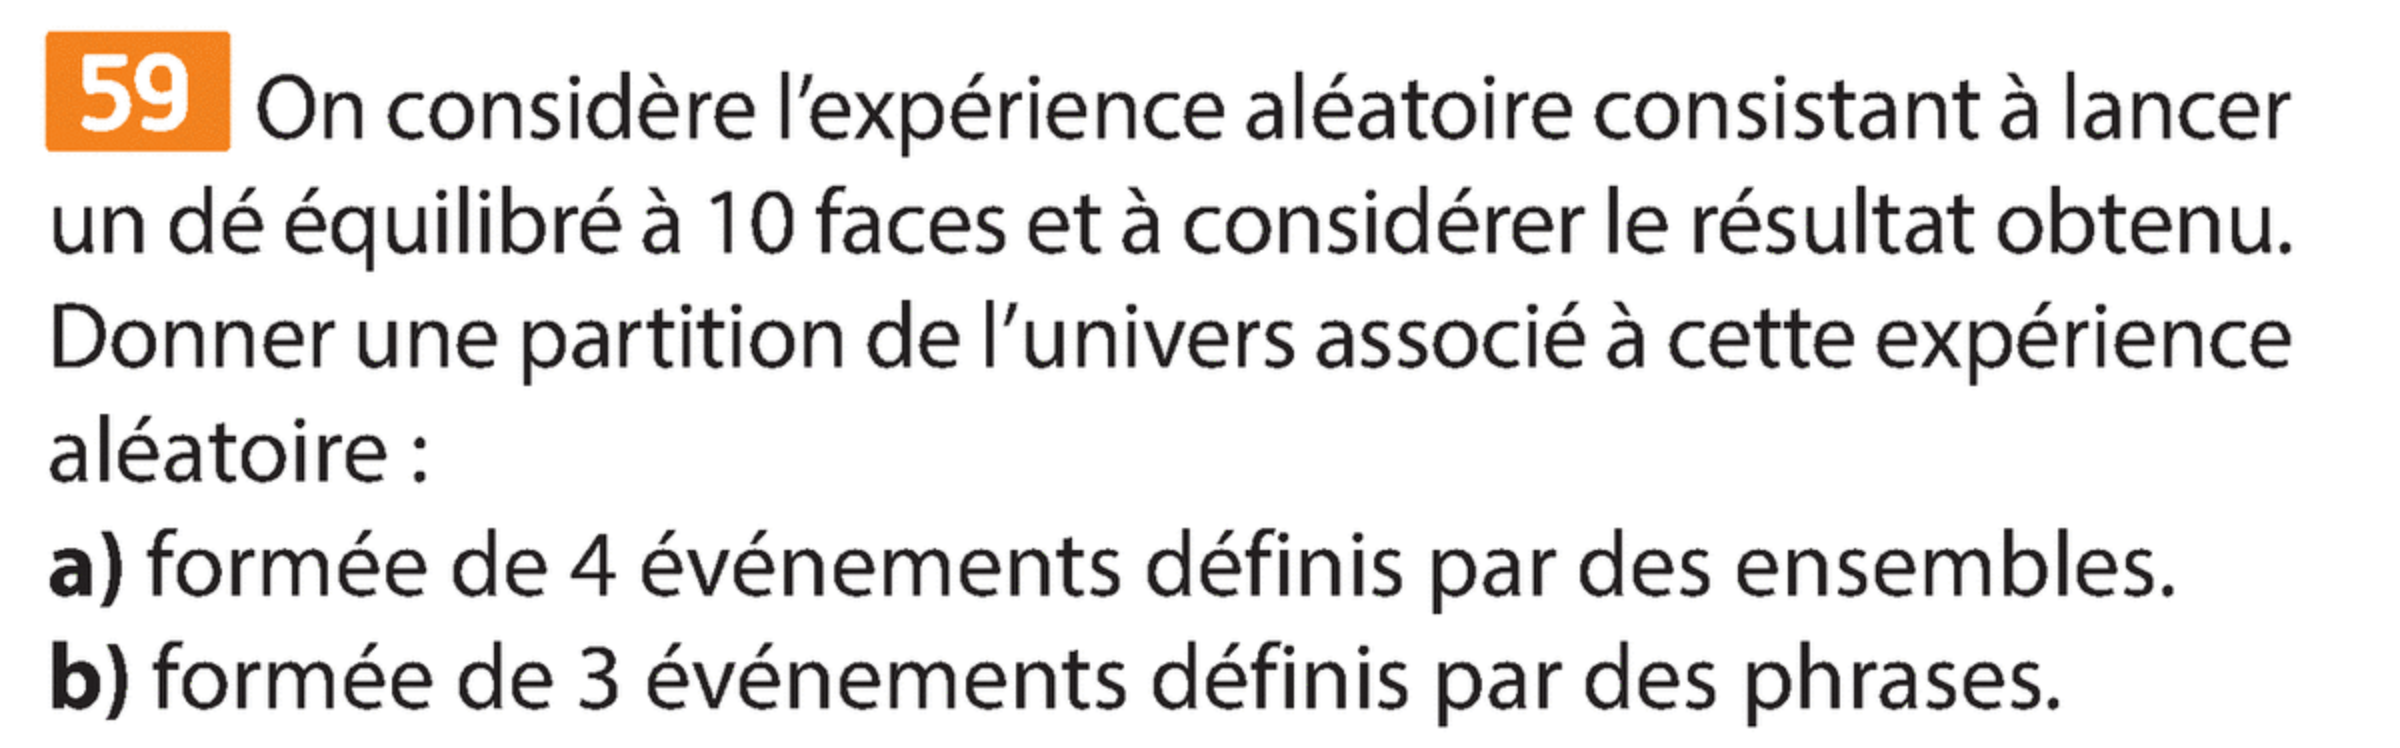
\includegraphics[width=\textwidth]{Exo_59.png}
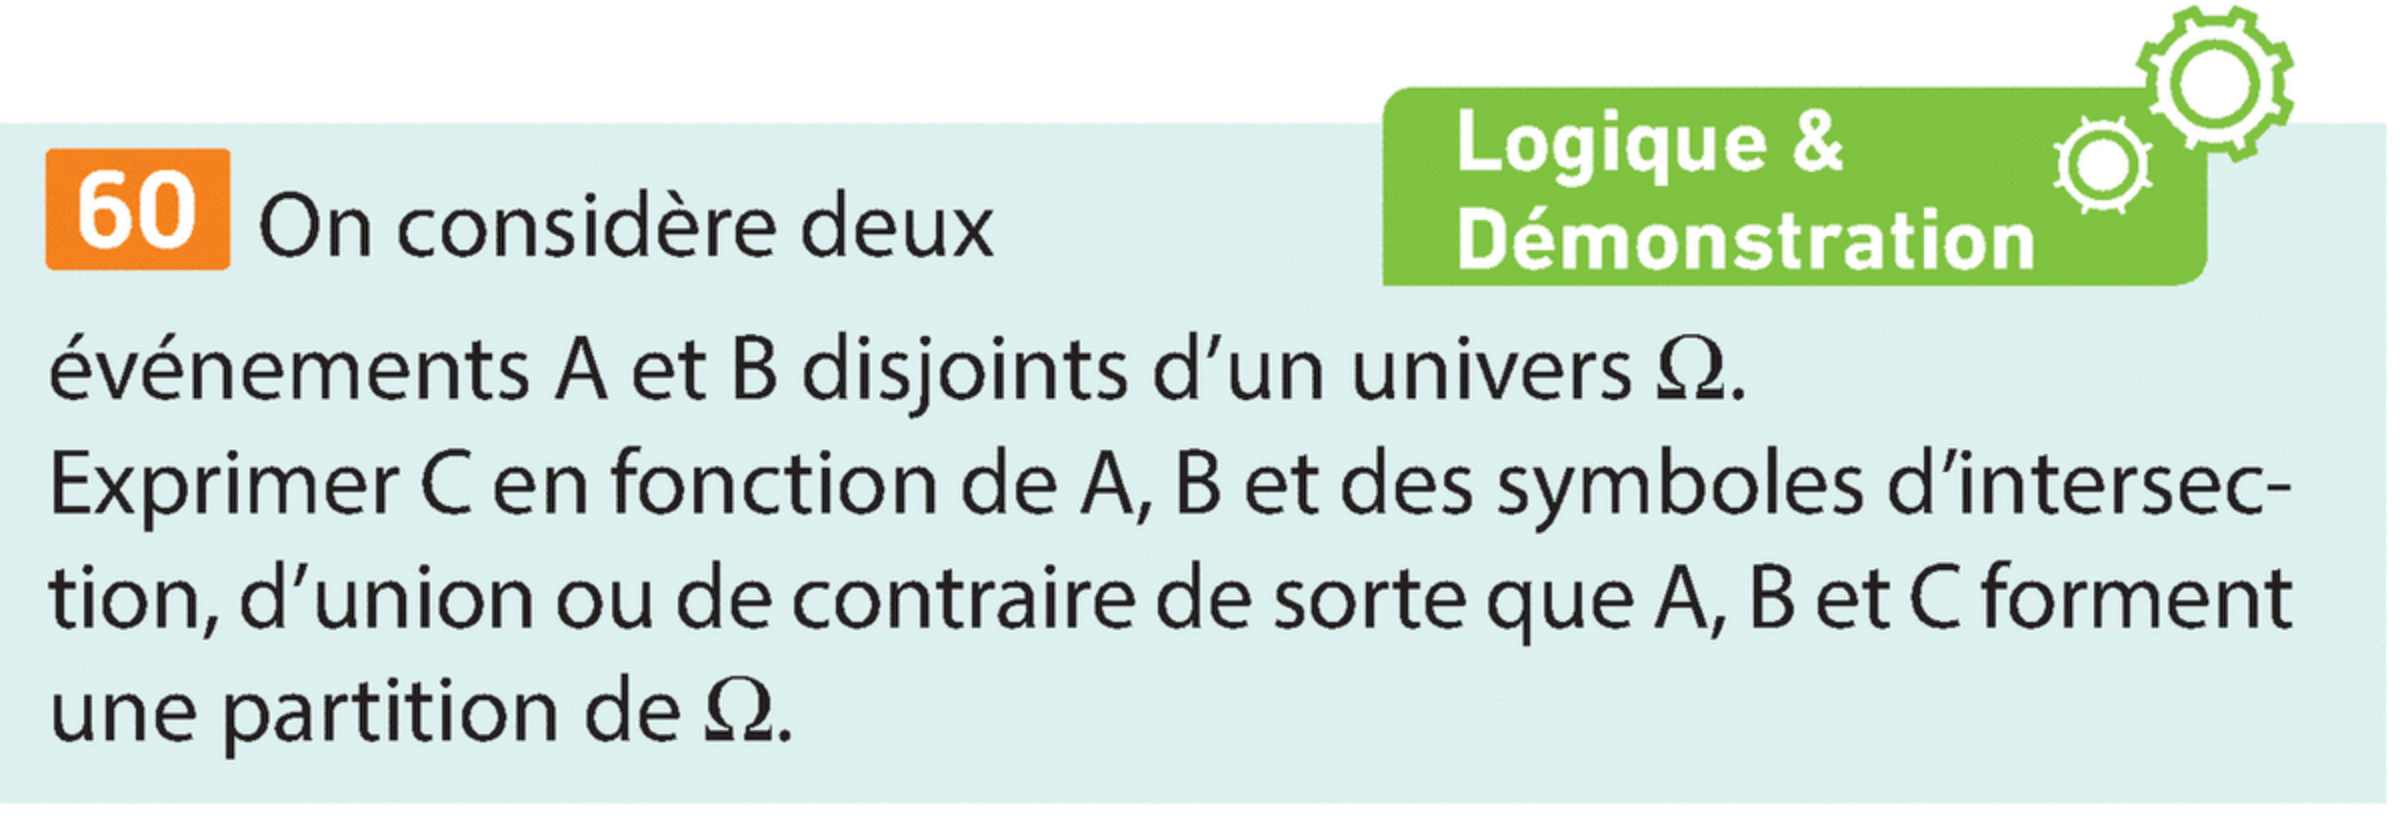
\includegraphics[width=\textwidth]{Exo_60.png}
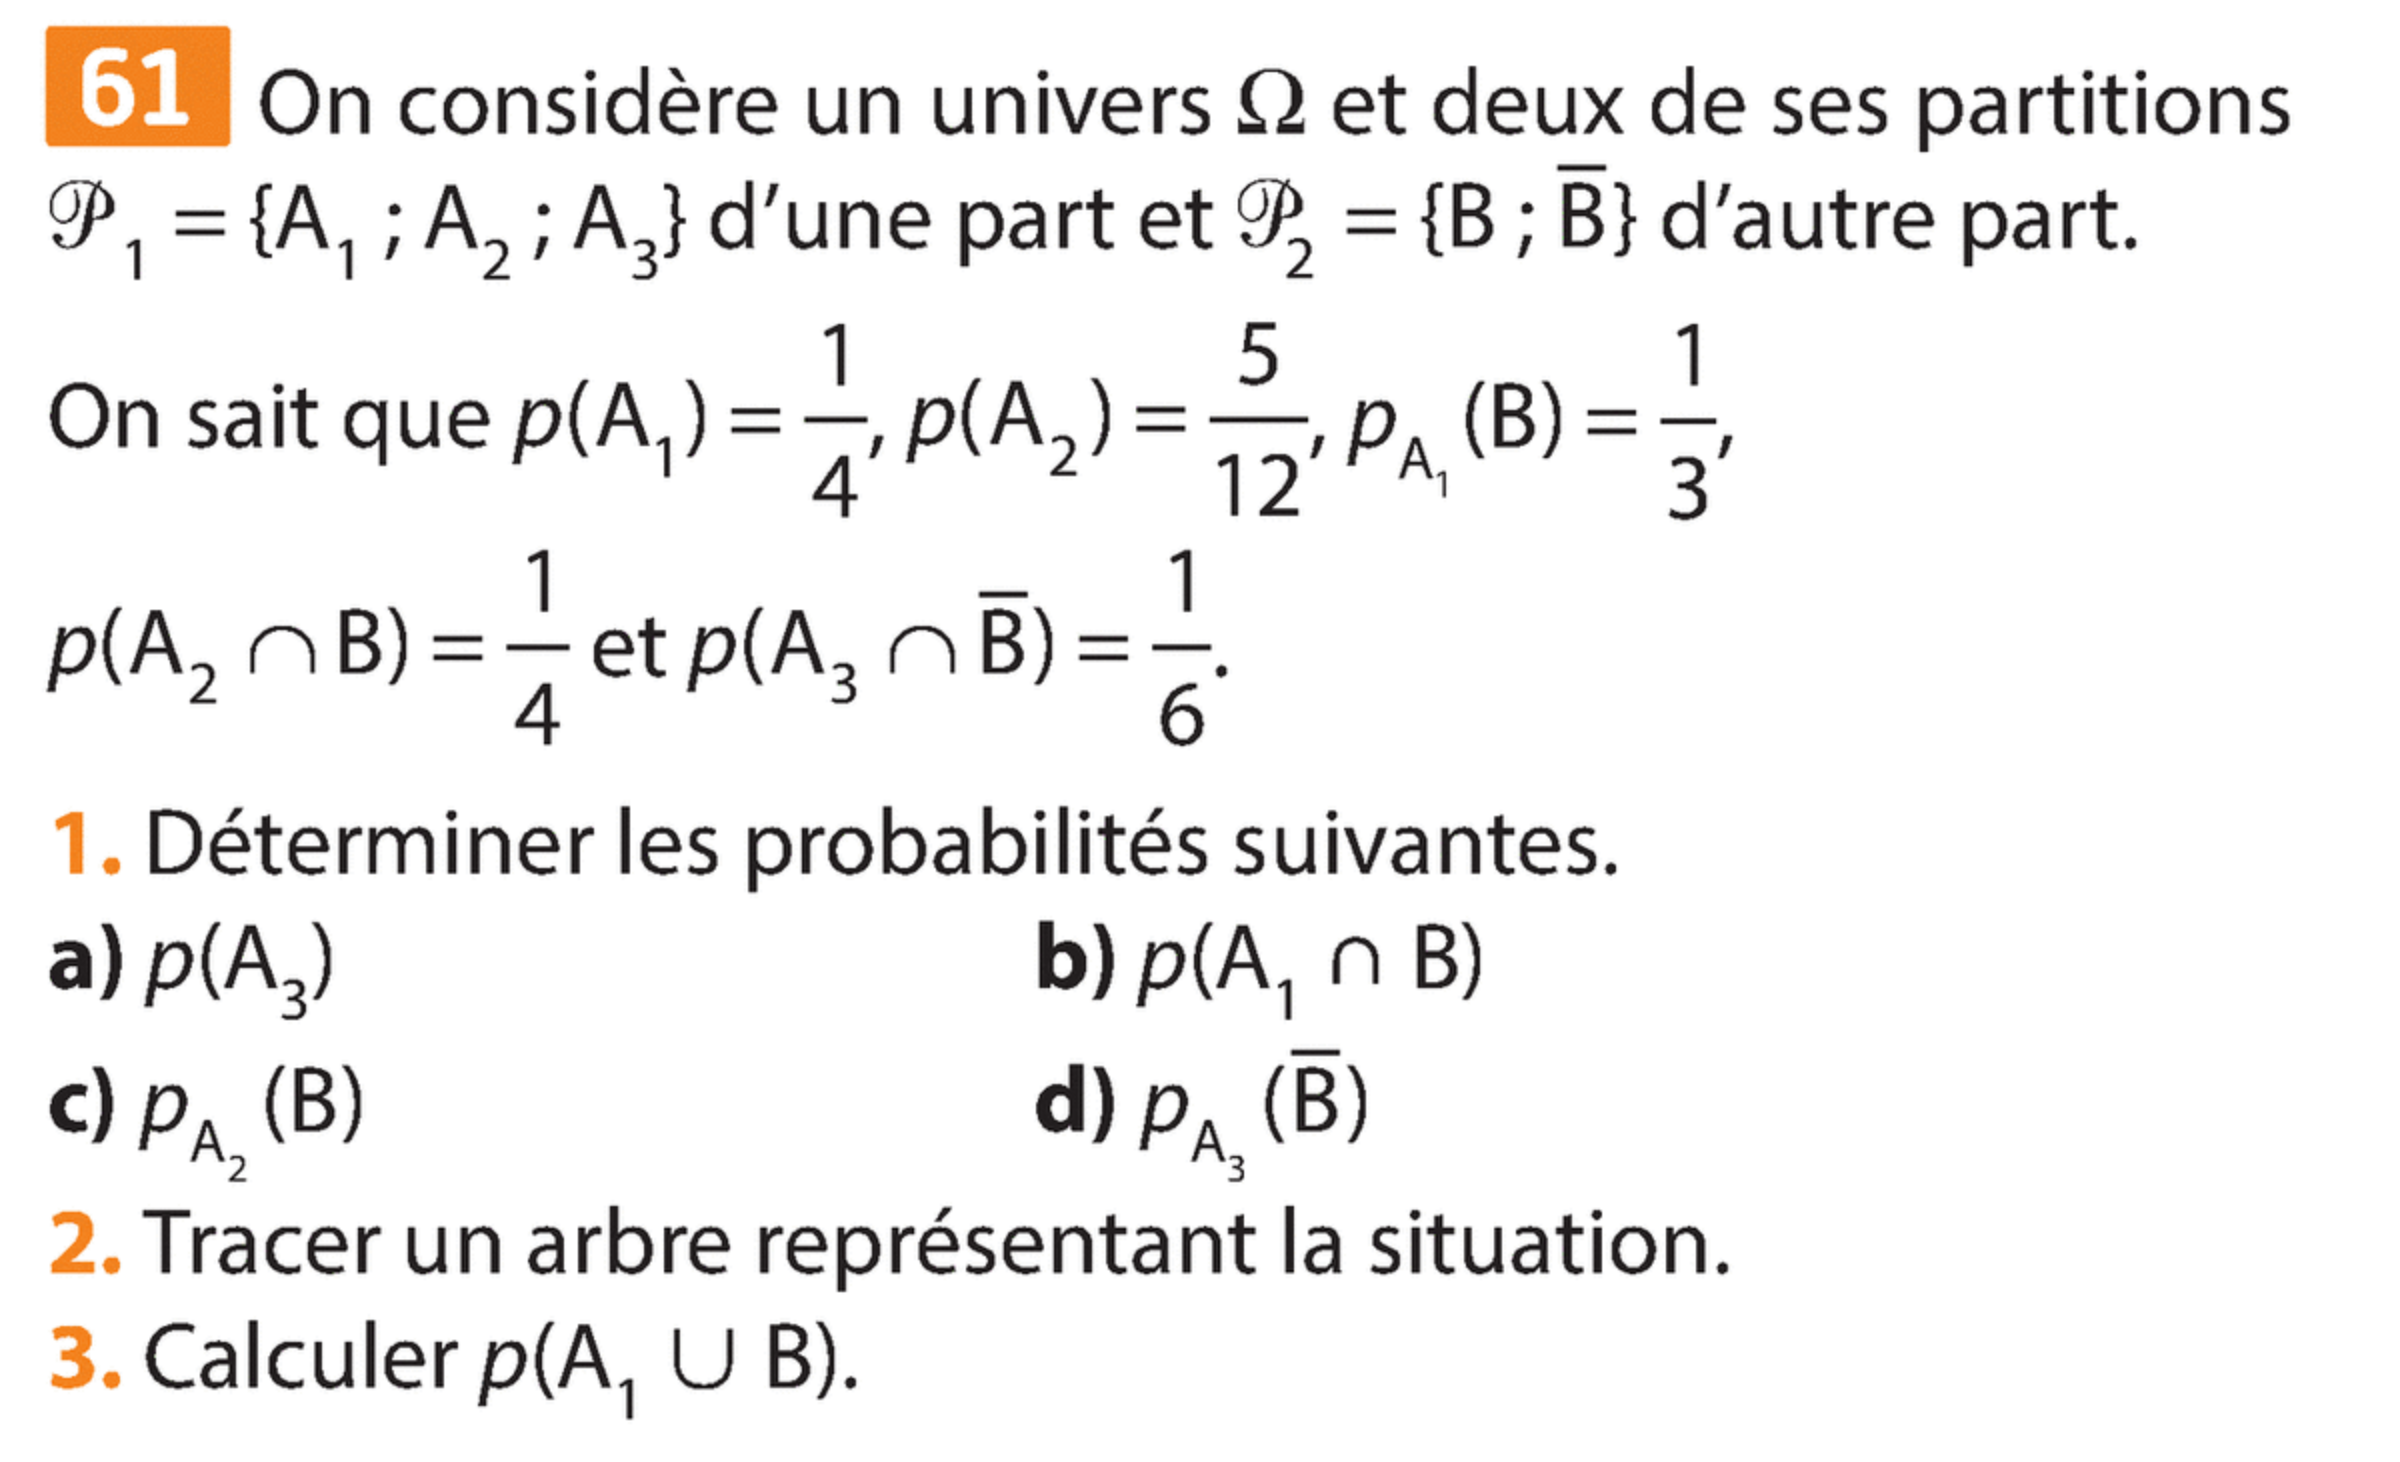
\includegraphics[width=\textwidth]{Exo_61.png}
\end{minipage}
\hfill\vline\hfill
\begin{minipage}[t]{0.45\textwidth}
\begin{center}
\textbf{Bilan sur les arbres}
\end{center}
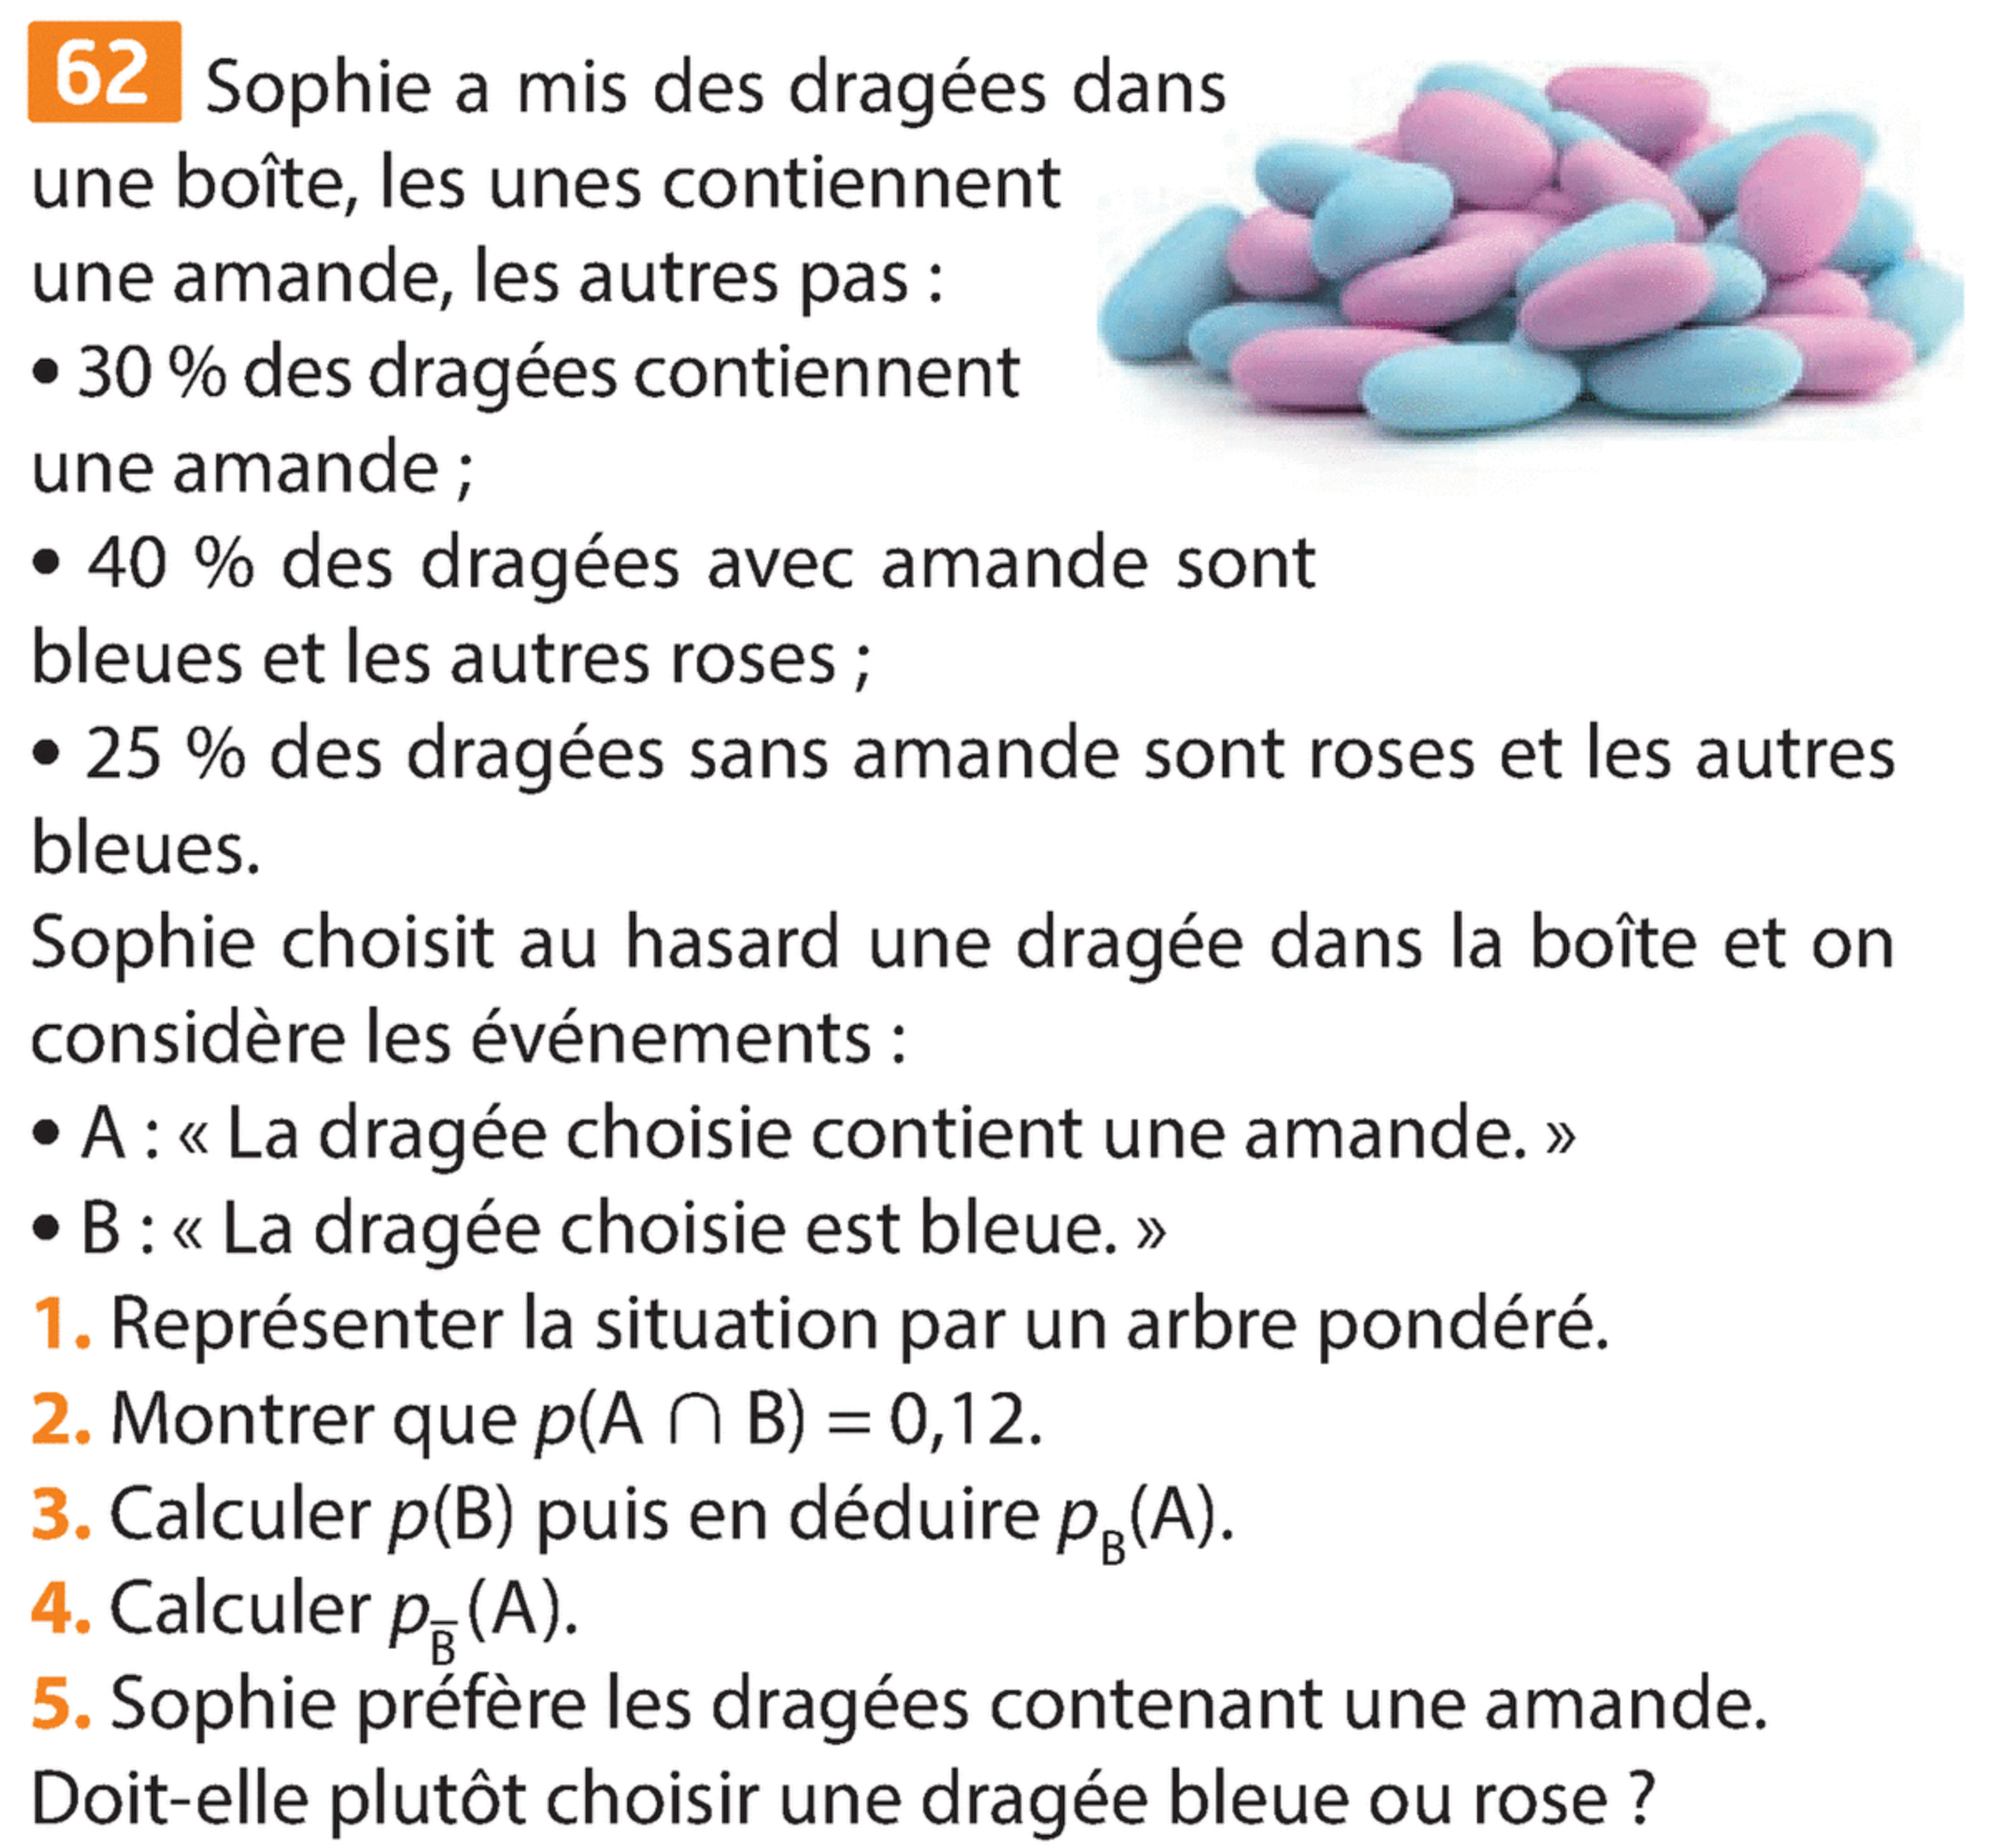
\includegraphics[width=\textwidth]{Exo_62.png}
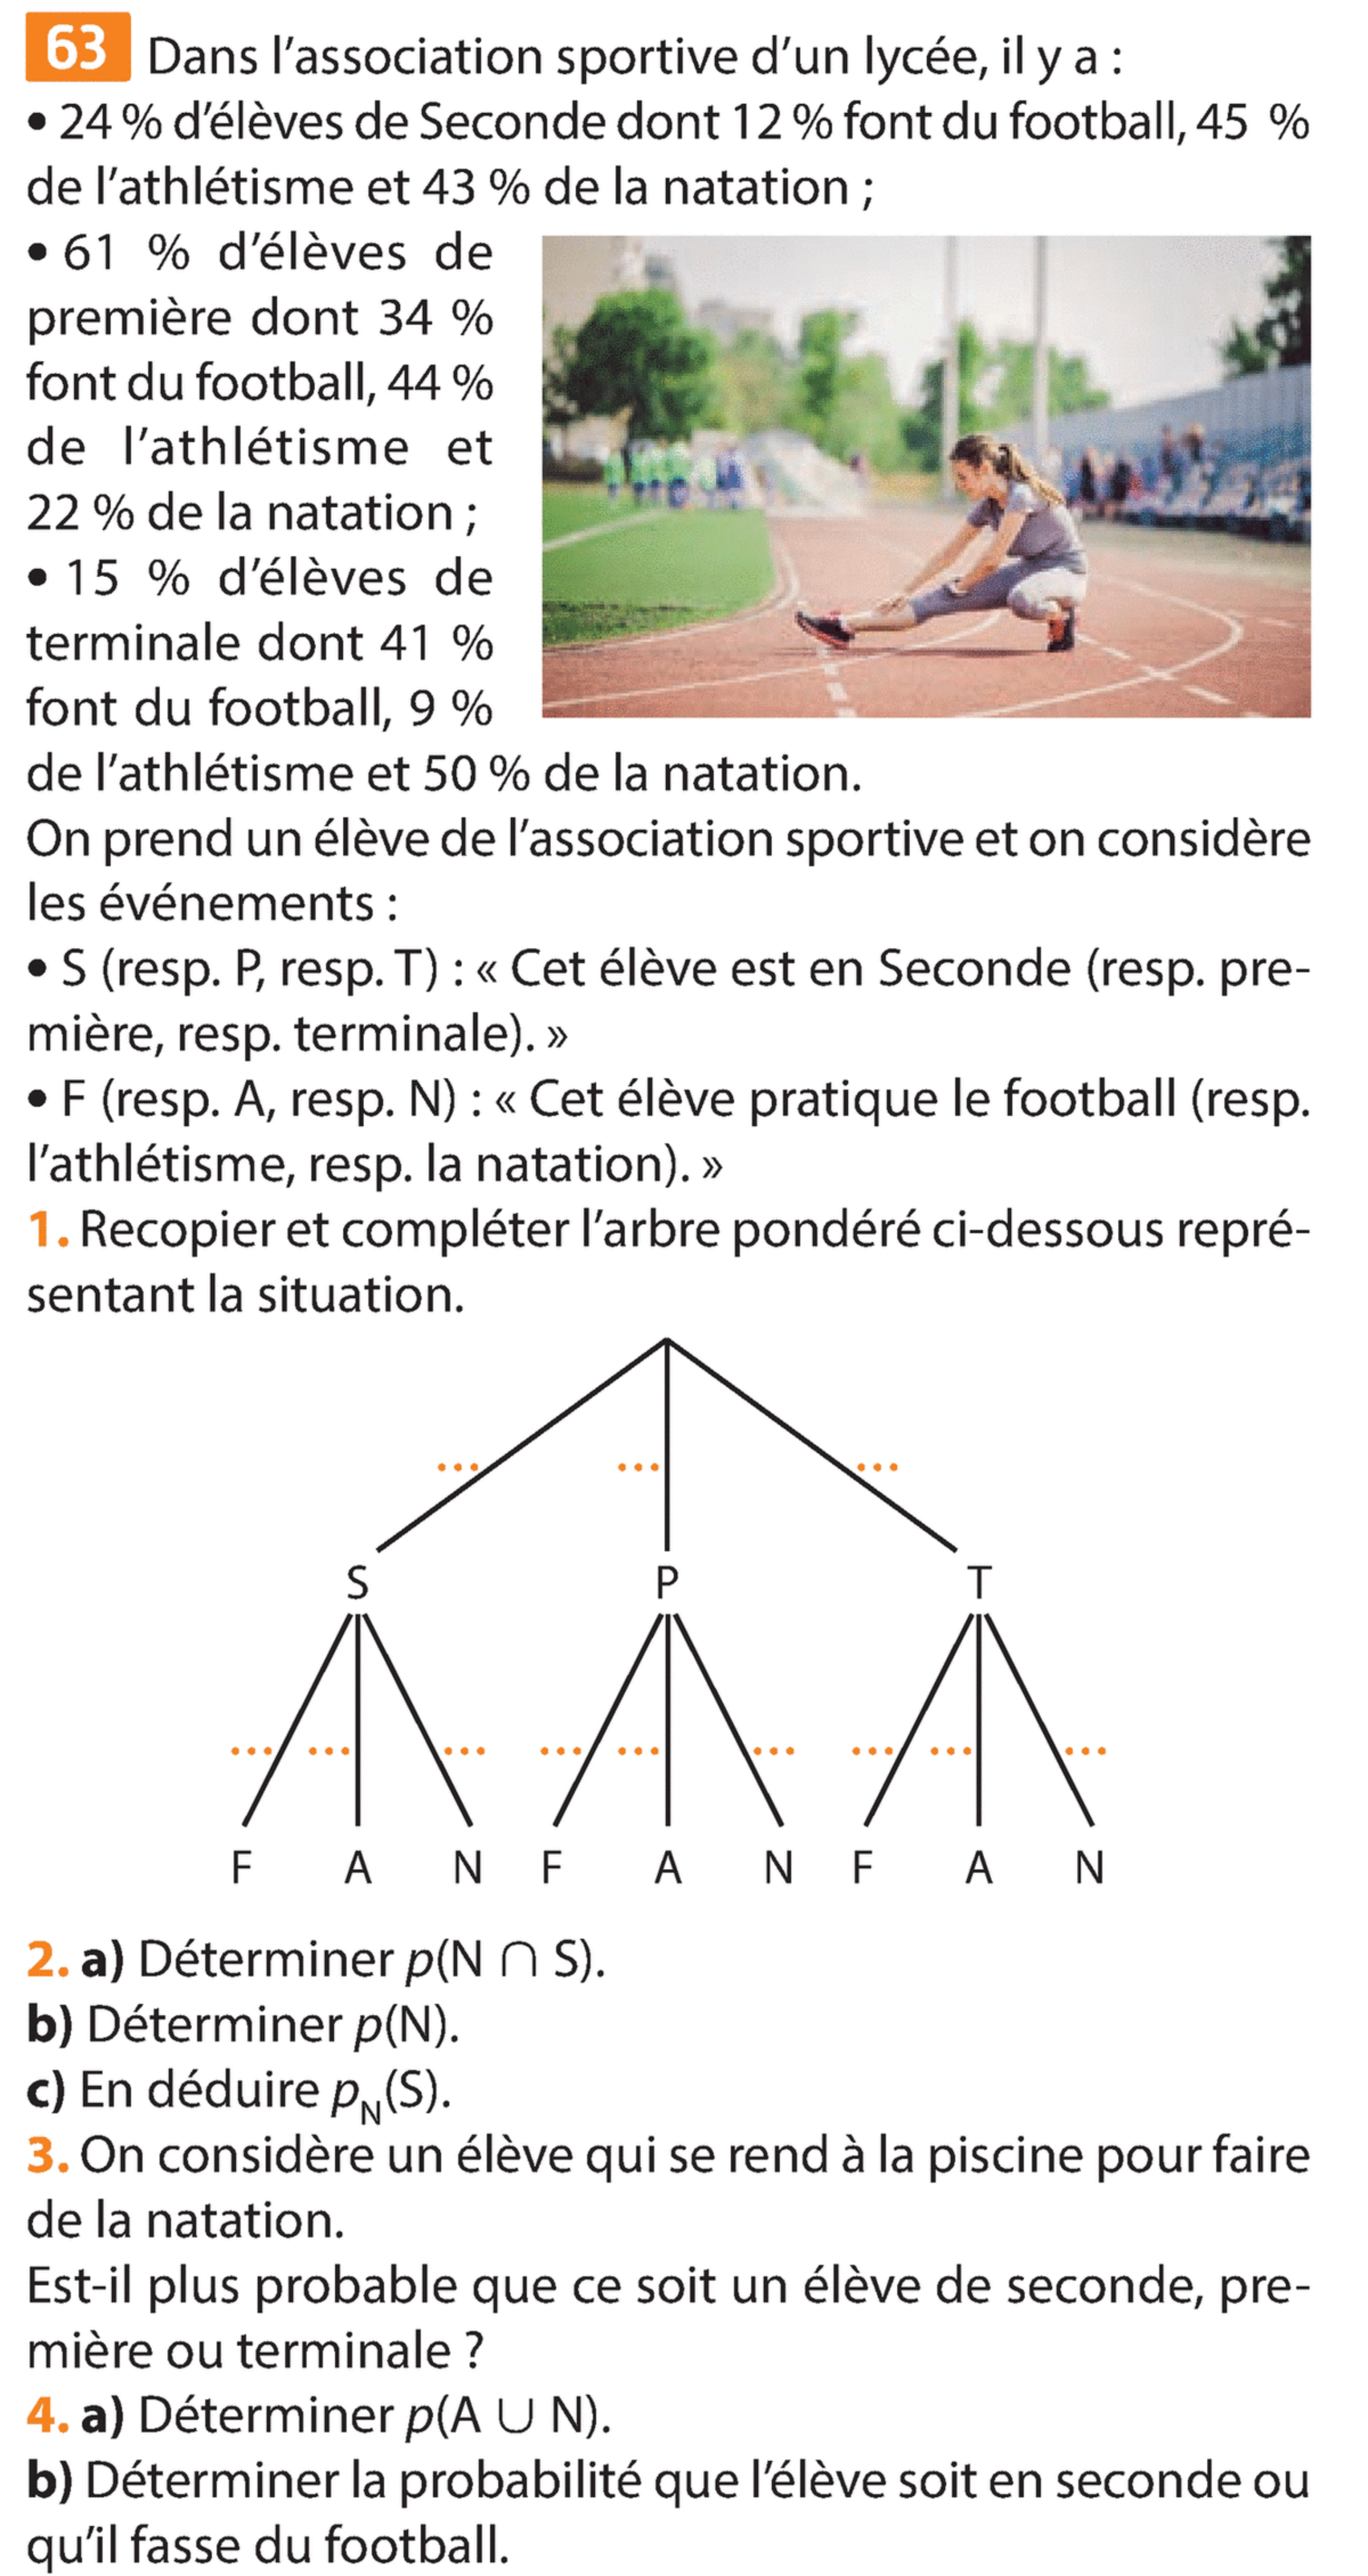
\includegraphics[width=\textwidth]{Exo_63.png}
\end{minipage}
\end{document}  